\chapter{Path tracing integrator and Next Event Estimation}
\label{chapter:ptdl}


\section{Path tracing and numerical stability issues}
\label{section:numerical}

Unbiased nature of the brute force volumetric path tracing estimator and
physically based parametrization makes it a almost perfect candidate for
implementing the reference integrator.
The inherent characteristic of the brute force volumetric pathtracing estimator
is a high variance, which leads to long rendering times in practice. Being
applicable in practice, variance reduction techniques usually emplyed. For
example Russian Roulette is one of them.

\begin{figure}[h]
    \centering
    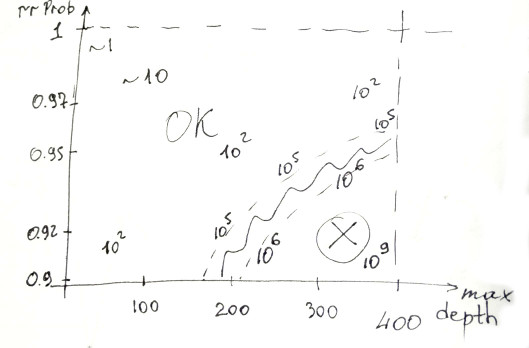
\includegraphics[width=0.75\textwidth]{imgs/plots/rr_heuristic_draft}
    \caption{Draft of the plot showing numerically instabile parameter regions}
    \label{fig:rr_regions}
\end{figure}

The use of Russian Roulette in the context of volumetric rendering may lead to
unexpected loss of energy during simulations. It is observed as the objects are
rendered darker than the in theory should.

The cause of this effect is the numerical cancellations which appear during
rendering high albedo materials with high scattering coefficients. 

It is possible to build heuristic approach to estimate the minimum allowed
Russian Roulette threshold parameter on the basis of the scattering properties
of the media. While still being sure that there is no energy is lost because of
numerical cancellation.

\ldots


\section{PTDL volume integrator}

Detailed description of the PTDL for volumetric path tracer.
Direct light sampling from inside the medium. Special case for each light
source. Energy conservation tests.


\section{Combining brute force path tracing volume integrator with PTDL. MIS}
It was not implemented yet. Low priority section.

\ldots